%%%%%%%%%%%%%%%%%%%%%%%%%%%%%%%%%%%%%%%%%%%%%%%%%%%%%%%%%%%%%%%%%%%%%%%%%%%%%%%%
%2345678901234567890123456789012345678901234567890123456789012345678901234567890
%        1         2         3         4         5         6         7         8

\documentclass[letterpaper, 10 pt, conference]{ieeeconf}  % Comment this line out
                                                          % if you need a4paper
%\documentclass[a4paper, 10pt, conference]{ieeeconf}      % Use this line for a4
                                                          % paper

\IEEEoverridecommandlockouts                              % This command is only
                                                          % needed if you want to
                                                          % use the \thanks command
\overrideIEEEmargins
% See the \addtolength command later in the file to balance the column lengths
% on the last page of the document

\usepackage[utf8]{inputenc}
\usepackage[T1]{fontenc}
\usepackage{graphicx}

% The following packages can be found on http:\\www.ctan.org
%\usepackage{graphics} % for pdf, bitmapped graphics files
%\usepackage{epsfig} % for postscript graphics files
%\usepackage{mathptmx} % assumes new font selection scheme installed
%\usepackage{mathptmx} % assumes new font selection scheme installed
%\usepackage{amsmath} % assumes amsmath package installed
%\usepackage{amssymb}  % assumes amsmath package installed

\title{\LARGE \bf
Machine Translation for Tibetan Buddhist Texts
}

%\author{ \parbox{3 in}{\centering Huibert Kwakernaak*
%         \thanks{*Use the $\backslash$thanks command to put information here}\\
%         Faculty of Electrical Engineering, Mathematics and Computer Science\\
%         University of Twente\\
%         7500 AE Enschede, The Netherlands\\
%         {\tt\small h.kwakernaak@autsubmit.com}}
%         \hspace*{ 0.5 in}
%         \parbox{3 in}{ \centering Pradeep Misra**
%         \thanks{**The footnote marks may be inserted manually}\\
%        Department of Electrical Engineering \\
%         Wright State University\\
%         Dayton, OH 45435, USA\\
%         {\tt\small pmisra@cs.wright.edu}}
%}

\author{ Jacob Atkins$^{1}$, Chris Calloway$^{2}$, Kelsey Namba$^{3}$, Rahul Sehrawat$^{4}$% <-this % stops a space
\thanks{*Smara Muresan, Isabelle Zuagg, Jonathan Reeve}% <-this % stops a space

}


\begin{document}



\maketitle
\thispagestyle{empty}
\pagestyle{empty}


%%%%%%%%%%%%%%%%%%%%%%%%%%%%%%%%%%%%%%%%%%%%%%%%%%%%%%%%%%%%%%%%%%%%%%%%%%%%%%%%
\begin{abstract}

(Rahul)

\end{abstract}


%%%%%%%%%%%%%%%%%%%%%%%%%%%%%%%%%%%%%%%%%%%%%%%%%%%%%%%%%%%%%%%%%%%%%%%%%%%%%%%%
\section{INTRODUCTION}

Digital language justice is the right for an user to use the language they are most comfortable with in the digital sphere. Language justice goes beyond this, however. With modern technology, it is possible to reconnect people with their cultural dispora. Our project aims to increase the accessibility of Tibetan religious texts by training a machine translation model specifically to translate religious Tibetan texts to English. We hope to create a translation device for Tibetan Buddhist practitioners who are non-Tibetan speakers, allowing them access to texts that had previously been barred by the language barrier. We have trained our model in PyTorch and have leveraged the BART architecture in the HuggingFrance transformers library to make the training and architecture more straightforward. By creating thesee models, we hope to motivate scholars to study not only these texts but Tibetan as a whole. Currently, while there has been some interest in machine translation for Tibetan-Chinese and vice versa, the same interest has not been reflected in Tibetan-English machine translation. From a deep dive into the open-source Tibetan NLP material, we were unable to find any projects attempting to translate Tibetan-English nor could we find papers specifically discussing Tibetan-English machine translation. By having a readily available set of translated discourses could create an on-ramp for further language uses because increased access could lead to increased interest, especially in the English-speaking community. 


\section{ETHICAL CONSIDERATIONS}

Care must be taken when approaching culturally and spiritually important texts for use in a computational domain. To that end we authors acknowledge our place as outsiders of the Buddhist tradition and outline our ethical approach for translating these texts as said outsiders.

First, we acknowledge that it would be improper to consider our translations as genuine sutras. No matter what our results are, we authors are not in a qualified position to declare something as an honest translation of a Tibetan Buddhist text. To that end, we have instead given our translations to someone who can give a more qualified opinion of the accuracy of our translation. In this case, we asked a Native Tibetan Speaker who holds a Master's degree in Buddhist theology and philosophy and a current PhD candidate in Tibetan History to  assess our results. This approach to invite someone directly in the Tibetan community to assess our results was inspired by Bird's paper \cite{c7} which suggests including a "human in the loop" as a key step in the process to decolonizing NLP research. 

Second, we acknowledge that there are certainly Indo-Tibetan texts that would be inappropriate to translate. These texts, namely the Tantric (esoteric) texts, we understand are meant for a select subset of advanced practitioners and translating these texts for the masses could be spiritually dangerous. Knowing this, we have refrained from including and Tantric texts within our training data.


Lastly, we acknowledge this is a tool to help bridge the language gap between practitioners both in and out of the Tibetan culture. We authors want to emphasize that this is just a tool. We make no claims that this tool will solve or fix the underlying social injustice issues within Tibetan community and diaspora. While we hope this tool can bring the community closer together and aid in prosperity, we make no claims that it will be able to do so. 

\section{PROCEDURE}



\subsection{Data and Pre-processing}

To train our model, we acquired publicly available English to Tibetan parallel corpuses. The non-profit 84000 provided 80 English to Tibetan parallel texts on their website \cite{c8}. All 80 of these texts were expert translations of Indo-Tibetan Buddhist texts. For our model we used all 80 of these provided texts.

Before using 84000's corpuses however, we pre-processed the provided data to meet our model's need. The provided files from 84000 were in a .tmx file format, a very standard parallel corpus file format \cite{c9}. 
For our approach, we scraped all 80 .tmx files for both its English and Tibetan contents and placed them line by line into two large .txt files. One .txt file contained the English lines, and the other .txt file contained the Tibetan translation. We made careful assurance that the lines remained in exactly one to one correspondence with their translations. That is, a newline character was used to distinguish two separate lines of translation, but the same line number in each file corresponds to the exact translation provided by 84000. Therefore, the total line numbers in the two .txt files were necessarily the same since one line in one file corresponding to exactly the same line of translated text in the other file. Two such .txt file were made for each of the 80 .tmx files, a Tibetan and an English .txt file for each. After all 160 .txt files were generated, two single large .txt file was generated by concatenating all the Tibetan .txt files and all the English .txt files. These last two .txt files are what was fed into the model.

TODO: Actually do this/remove following lines. It was not strictly necessary to separate the creation of the large .txt files into the smaller components. However, giving the limited data we had this method proved useful to see how much individual texts contributed to the model (ie by eliminating some texts in some runs). 



\subsection{Model Design}
We used a 6 layer Transformer model that used a multi headed attention mechanism and a switchout transform. Each layer of the transformer model can be divided into an encoder and decoder layer. The encoding layer consists first of a self attention layer, an attention aspect which focuses on the encoded sentence, and then outputs to a feed forward layer. The multi part of the multi headed attention means that each head will encode the information in parallel and then the results will be concatenated and passed to the decoder. Figure one demonstrates this process.
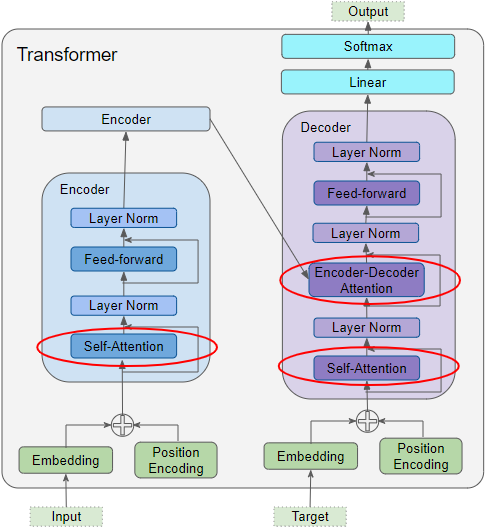
\includegraphics[scale=.4]{Transformer.png}
\caption{\\Figure 1: Overview of a Transformer model}
\\
\par
To prevent overfitting and to augment the data, we added in a switchout transform which will randomly switch out words in the source and target sentence. This also has the added advantage of augmenting the data even further which is especially important for our problem as religious tibetan has a relatively small corpus, around 30 thousand words. We also attempted to use masking, however we found it to be ineffective. Masking hides tokens from the model by replacing the tokens with a <mask> token. Tibetan tokens are not separated in the same way that latin languages separate their tokens. For example,
\begin{verbatim}
“བྱང་ཆུབ་མངོན་པར་རྫོགས་པར་འཚང་རྒྱ་སྟེ།” 
\end{verbatim}
a line in our test corpus translates to “Having the altruistic intention of excellent bodhicitta.” The tibetan word is only one token. Therefore, the mask would not help the model learn at all, as the entire sentence would be marked as <mask> and there would not be enough context for our model to discover the meaning. As a result, we did not use any form of masking in our model. Switchout does not create the same problem as their is always a token to take its place. \par
After implementing our transformer model with switchout we tuned hyper parameters to maximize our Transformer model. We manually tuned the following hyperparameters: dropout, label smoothing, rnn size, the number of transformer layers and the number of heads of the attention model. The final configuration used can be found in the appendix. \par
We used four different metrics to evaluate our results: accuracy, predicted score, perplexity and bilingual evaluation understudy (BLEU). The validation accuracy tells us how well we are learning our training data, the predicted score tells us the average log likelihood for each word, the perplexity tells us how well the model predicts the data and the bleu score evaluates the quality of the translation. Together, these metrics provide us with a decent picture of how well our model is performed. 

\section{Results}
\begin{tabular}{ |c| c| c| c| }
 Validation & Ave. Pred. Score & PPL & BLEU \\ 
 40.32\% & -1.69 & 5.41 & 23.01\% \\

\end{tabular}\\

\par
Our six layer transformer model with switch out was unsuccessful at translating religious tibetan to english. The translated output does not match closely enough in either pure accuracy or in the meaning of the passage to be useful in translating religious tibetan texts to english. \par
While superficially, the perplexity appears to demonstrate a strong model, further investigation demonstrates that the low perplexity is a sign of inaccuracy. Perplexity measures the number of possible words that a model could predict for any given sentence. A higher perplexity indicates higher uncertainty. However, the low BLEU score, which measures the quality of the machine translation, has already demonstrated that the accuracy is low. This combined with the perplexity shows the models overconfidence in predicting certain phrases. For example, the tibetan phrase །དེ་ནས་བཅོམ་ལྡན་འདས་ལ་བྱང་ཆུབ་སེམས་དཔའ་སེམས་དཔའ་ཆེན་པོ་བྱམས་པས་འདི་སྐད་ཅེས་གསོལ་ཏོ། translates to “So the bodhisattva mahāsattva Maitreya asked the Blessed One”, but the top five of the predicted translations all are of the form “The Blessed One then said to the [adj] [proper noun]”. Even though this sentence is wrong, the perplexity is low because the model is confident in the first part of the sentence. This phenomenon is repeated throughout the results. Keyphrases from the Tibetan sentence are interpreted wrongly in the same way, and then the model learns to be confident about its predictions which lowers the perplexity. \par
The results demonstrate the flaw in the Transformer model using the current parallel Tibetan to English corpuses. Each token in the Tibetan sentence corresponds to an entire phrase in english rather than a separate word. This complicates the translation, and the model learns parts of the phrases quite well. The validation accuracy is relatively high because the transformer model is good at learning parts of these phrases but it is not good at learning entire sentences or stringing together sentences in context which contributes to the low BLEU score. Overall, the model is capable of learning specific phrases well, but fails at the broad task of creating coherent translations from religious tibetan texts to english.


\section{Discussion}

Considering our use of word segmentation for preprocessing our data (as opposed to character segmentation), our results are comparable with, albeit lower than, Tibetan-Chinese models. Lai, Zhao, and Bao ran several different Tibetan-Chinese models on the same data using two different preprocessing methodologies, character segmentation and word segmentation. Their word segmented Transformer model averaged a higher BLEU score than ours, scoring a 38.44\% while our model scored 23.01\%. 

(Kelsey)



\section{Conclusion}


(Rahul)


\section*{APPENDIX}

Appendixes should appear before the acknowledgment. (not sure what we even need to put here ~Chris)

\section*{ACKNOWLEDGMENT}

The authors would like to thank Palden Gal for volunteering to read our translated texts. We would also like to thank Smara Muresan, Isabelle Zuagg, and Jonathan Reeve for mentoring this research. Lastly, we would like to thank the 84000 project for providing open source parallel Tibetan corpuses. 


(Chris)
\begin{thebibliography}{99}



\bibitem{c1} Cai Z. (2015) A Method for the Chinese-Tibetan Machine Translation System’s Syntactic Analysis. In: Wong W. (eds) Proceedings of the 4th International Conference on Computer Engineering and Networks. Lecture Notes in Electrical Engineering, vol 355. Springer, Cham. 

\bibitem{c2} Liu, H., Zhao, W., Yu, X., & Wu, J. (2016). A Chinese to Tibetan Machine Translation System with Multiple Translating Strategies. Himalayan Linguistics, 15(1).

\bibitem{c3} Hill, Nathan & Meelen, Marieke. (2017). Segmenting and POS tagging Classical Tibetan using a Memory-Based Tagger. Himalayan Linguistics. 16. 10.5070/H916234501. 

\bibitem{c4} Faggionato, Christian  and Meelen, Marieke. (2019). Developing the Old Tibetan Treebank. INCOMA Ltd. Proceedings of the International Conference on Recent Advances in Natural Language Processing (RANLP 2019) 304--312


\bibitem{c5} Orna Almogi, Lena Dankin, Nachum Dershowitz, Lior Wolf. A Hackathon for Classical Tibetan.Journal of Data Mining and Digital Humanities, Episciences.org, 2019, Special Issue on Computer-Aided Processing of Intertextuality in Ancient Languages. hal-01371751v3

\bibitem{c6} Orna Almogi, Lena Dankin, Nachum Dershowitz, Lior Wolf. A Hackathon for Classical Tibetan.Journal of Data Mining and Digital Humanities, Episciences.org, 2019, Special Issue on Computer-Aided Processing of Intertextuality in Ancient Languages. hal-01371751v3


\bibitem{c7} Bird, S. (2020). Decolonising Speech and Language Technology. Proceedings of the 28th International Conference on Computational Linguistics (COLING 2020), 3504–3519.


\bibitem{c8} 84000 Project (2021). What We Do. https://84000.co/about/what-we-do


\bibitem{c9} Coverpages (1997). TMX Format. http://xml.coverpages.org/tmxSpec971212.html




\end{thebibliography}




\end{document}


